\documentclass{beamer}

\usepackage[utf8]{inputenc}
\usepackage{fancybox,fancyvrb}
\usepackage{environ}
\usepackage{tikz}

\beamertemplatenavigationsymbolsempty
\setbeamertemplate{footline}[frame number]
\usetheme{Pittsburgh}

\newcommand\enumnum[1]{{\renewcommand{\insertenumlabel}{#1}%
      \usebeamertemplate{enumerate item} \,}}

\newcommand{\grad}{\nabla}
\newcommand{\ih}{\boldsymbol{\hat{\textbf{\i}}}}
\newcommand{\jh}{\boldsymbol{\hat{\textbf{\j}}}}
\newcommand{\vF}{\boldsymbol{\vec{\textbf{F}}}}
\newcommand{\Matlab}{\textsc{Matlab}}


\title{5.1 Linear mass-spring models}

\subtitle{a lesson for MATH F302 Differential Equations}

\author{Ed Bueler, Dept.~of Mathematics and Statistics, UAF}

\date{\tiny \today}


\begin{document}
\setbeamertemplate{itemize item}{$\bullet$}
\setbeamertemplate{itemize subitem}{$\circ$}


\begin{frame}
\titlepage

\centerline{\tiny for textbook: \, D. Zill, \emph{A First Course in Differential Equations with Modeling Applications}, 11th ed.}
%\color{green!40!blue}
\end{frame}


\begin{frame}{a good reason}

\begin{itemize}
\item in Chapter 4 we've spent time solving 2nd-order linear DEs
    $$a y'' + b y' + c y \stackrel{\ast}{=} g(t)$$
\item a good reason is that

\medskip
\centerline{\alert{anything that smoothly oscillates has DE $\ast$ for a model}}

    \begin{enumerate}
    \item a mass suspended on a spring oscillates up and down
    \item the current in a radio-type circuit flows back-and-forth
    \item a pendulum swings back and forth
    \item the earth moves up and down in an earthquake
    \item magnetic field in a radio wave oscillates
    \item a drum-head vibrates
    \item a photon is
    \end{enumerate}

\item my 5.1 and 5.3 slides take \enumnum{1}--\enumnum{3} seriously
\end{itemize}
\end{frame}


\begin{frame}{setting up the mass-spring}

careful set-up so that the equations are clear:
\begin{columns}
\begin{column}{0.6\textwidth}
\begin{itemize}
\small
\item choose spring with relaxed length $\ell$ and spring constant $k$
\item hang it from rigid support
\item choose mass $m$ and hook to the spring
\item let it down to its equilibrium position; it has stretched by $s$
\item set a scale next to the mass-spring with $x=0$ at equilibrium position and positive $x$ downward
\item thus $x$, the displacement when you move the spring, is the \emph{amount the spring has stretched (downward) from its equilibrium position}
\end{itemize}
\end{column}
\begin{column}{0.4\textwidth}
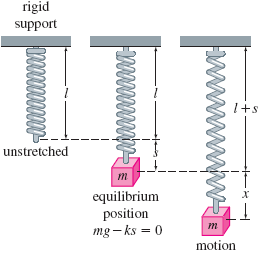
\includegraphics[width=\textwidth]{figs/mass-spring-setup}
\end{column}
\end{columns}
\end{frame}


\begin{frame}{Newton's law}

\begin{columns}
\begin{column}{0.65\textwidth}
\begin{itemize}
\item Newton's second law is $ma=F$
\item for our mass-spring system:

\vspace{-3mm}
    $$m \frac{d^2x}{dt^2} = - k x$$

\vspace{-2mm}
\item really:

\vspace{-2mm}
        $$m \frac{d^2x}{dt^2} = mg - k (x+s)$$

\vspace{-2mm}
    \begin{itemize}
    \item \dots but $mg=ks$
    \item in practice $k$ is \emph{determined} from $k=mg/s$
    \end{itemize}

\vspace{3mm}

\item ``Hooke's law'' $F_{spring} = -kx$ is a \emph{model} for how springs work
    \begin{itemize}
    \item not a bad model
    \item \dots for smallish displacements
    \item improved model 5.3
    \end{itemize}
\end{itemize}
\end{column}
\begin{column}{0.35\textwidth}
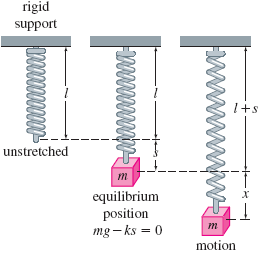
\includegraphics[width=\textwidth]{figs/mass-spring-setup}
\end{column}
\end{columns}
\end{frame}


\begin{frame}{first solution}

\begin{itemize}
\item from last slide the DE for our mass-spring:
    $$m \frac{d^2x}{dt^2} + k x = 0$$
\item it is constant coefficient so substitute $x(t)=e^{rt}$
\item get auxiliary equation
    $$m r^2 + k = 0$$
\item solutions are imaginary: $r = \pm \sqrt{\frac{k}{m}} i$
    \begin{itemize}
    \item X
    \end{itemize}
\end{itemize}
\end{frame}




\begin{frame}{exercise \#3 in \S5.1}

\begin{itemize}
\item X
\end{itemize}
\end{frame}


\begin{frame}{X}

\begin{itemize}
\item X
\end{itemize}
\end{frame}


\begin{frame}{X}

\begin{itemize}
\item X
\end{itemize}
\end{frame}


\begin{frame}{X}

\begin{itemize}
\item X
\end{itemize}
\end{frame}


\begin{frame}{forms}

\begin{tabular}{r|c|c}
 & Newton's law form & $\omega$ form \\ \hline \hline
\huge \strut \normalsize          undamped & $m \frac{d^2x}{dt^2} = - k x$ & $\frac{d^2x}{dt^2} + \omega^2 x=0$ \\ \hline
\huge \strut \normalsize            damped & $m \frac{d^2x}{dt^2} = - k x - \beta \frac{dx}{dt}$ & $\frac{d^2x}{dt^2} + 2 \lambda \frac{dx}{dt} + \omega^2 x=0$ \\ \hline
\huge \strut \normalsize \begin{tabular}{c} damped \\ and driven \end{tabular} & \small $m \frac{d^2x}{dt^2} = - k x - \beta \frac{dx}{dt} + f(t)$ & \small $\frac{d^2x}{dt^2} + 2 \lambda \frac{dx}{dt} + \omega^2 x=F(t)$ \\
\end{tabular}

$\omega=\sqrt{k/m}$

$\lambda = \beta / (2m)$

undamped solution:
    $$x(t) = c_1 \cos \omega t + c_2 \sin \omega t = A \sin(\omega t + \phi)$$
\end{frame}


\begin{frame}{damping cases}

$$\frac{d^2x}{dt^2} + 2 \lambda \frac{dx}{dt} + \omega^2 x=0$$

\begin{itemize}
\item \emph{undamped} if $\lambda = 0$
\item \emph{overdamped} if $\lambda^2-\omega^2 > 0$
\item \emph{critically damped} if $\lambda^2-\omega^2 = 0$
\item \emph{underdamped} if $\lambda^2-\omega^2 < 0$
\end{itemize}
\end{frame}



\begin{frame}{X}

\begin{itemize}
\item X
\end{itemize}
\end{frame}


\begin{frame}[fragile]
\frametitle{a plotting code: \texttt{massspringplot.m}}

\VerbatimInput[fontsize=\scriptsize]{../codes/massspringplot.m}
\end{frame}


\begin{frame}{circuit analogy}

\begin{itemize}
\item X
\end{itemize}

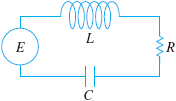
\includegraphics[width=0.4\textwidth]{figs/rlc-circuit}
\end{frame}


\begin{frame}{X}

\begin{itemize}
\item X
\end{itemize}
\end{frame}


\begin{frame}{expectations}

\begin{itemize}
\item just watching this video is \emph{not} enough!
     \begin{itemize}
     \item see ``found online'' videos at

     \centerline{\href{https://bueler.github.io/math302/week8.html}{\tt \color{cyan} bueler.github.io/math302/week8.html}}
     \item \emph{read} section 5.1 in the textbook
         \begin{itemize}
         \item material on ``double spring systems'' (p.~201) can be skipped
         \item while I discussed electrical circuits in these slides, I will not ask about it on quizzes or exams
         \end{itemize}
     \item \emph{do} the WebAssign exercises for section 5.1
     \end{itemize}
\end{itemize}
\end{frame}

\end{document}

